\documentclass[11pt,compress,t,notes=noshow, xcolor=table]{beamer}
\usepackage[]{graphicx}\usepackage[]{color}
% maxwidth is the original width if it is less than linewidth
% otherwise use linewidth (to make sure the graphics do not exceed the margin)
\makeatletter
\def\maxwidth{ %
  \ifdim\Gin@nat@width>\linewidth
    \linewidth
  \else
    \Gin@nat@width
  \fi
}
\makeatother

\definecolor{fgcolor}{rgb}{0.345, 0.345, 0.345}
\newcommand{\hlnum}[1]{\textcolor[rgb]{0.686,0.059,0.569}{#1}}%
\newcommand{\hlstr}[1]{\textcolor[rgb]{0.192,0.494,0.8}{#1}}%
\newcommand{\hlcom}[1]{\textcolor[rgb]{0.678,0.584,0.686}{\textit{#1}}}%
\newcommand{\hlopt}[1]{\textcolor[rgb]{0,0,0}{#1}}%
\newcommand{\hlstd}[1]{\textcolor[rgb]{0.345,0.345,0.345}{#1}}%
\newcommand{\hlkwa}[1]{\textcolor[rgb]{0.161,0.373,0.58}{\textbf{#1}}}%
\newcommand{\hlkwb}[1]{\textcolor[rgb]{0.69,0.353,0.396}{#1}}%
\newcommand{\hlkwc}[1]{\textcolor[rgb]{0.333,0.667,0.333}{#1}}%
\newcommand{\hlkwd}[1]{\textcolor[rgb]{0.737,0.353,0.396}{\textbf{#1}}}%
\let\hlipl\hlkwb

\usepackage{framed}
\makeatletter
\newenvironment{kframe}{%
 \def\at@end@of@kframe{}%
 \ifinner\ifhmode%
  \def\at@end@of@kframe{\end{minipage}}%
  \begin{minipage}{\columnwidth}%
 \fi\fi%
 \def\FrameCommand##1{\hskip\@totalleftmargin \hskip-\fboxsep
 \colorbox{shadecolor}{##1}\hskip-\fboxsep
     % There is no \\@totalrightmargin, so:
     \hskip-\linewidth \hskip-\@totalleftmargin \hskip\columnwidth}%
 \MakeFramed {\advance\hsize-\width
   \@totalleftmargin\z@ \linewidth\hsize
   \@setminipage}}%
 {\par\unskip\endMakeFramed%
 \at@end@of@kframe}
\makeatother

\definecolor{shadecolor}{rgb}{.97, .97, .97}
\definecolor{messagecolor}{rgb}{0, 0, 0}
\definecolor{warningcolor}{rgb}{1, 0, 1}
\definecolor{errorcolor}{rgb}{1, 0, 0}
\newenvironment{knitrout}{}{} % an empty environment to be redefined in TeX

\usepackage{alltt}
\newcommand{\SweaveOpts}[1]{}  % do not interfere with LaTeX
\newcommand{\SweaveInput}[1]{} % because they are not real TeX commands
\newcommand{\Sexpr}[1]{}       % will only be parsed by R



\usepackage[english]{babel}
\usepackage[utf8]{inputenc}

\usepackage{dsfont}
\usepackage{verbatim}
\usepackage{amsmath}
\usepackage{amsfonts}
\usepackage{bm}
\usepackage{csquotes}
\usepackage{multirow}
\usepackage{longtable}
\usepackage{booktabs}
\usepackage{enumerate}
\usepackage[absolute,overlay]{textpos}
\usepackage{psfrag}
\usepackage{algorithm}
\usepackage{algpseudocode}
\usepackage{eqnarray}
\usepackage{arydshln}
\usepackage{tabularx}
\usepackage{placeins}
\usepackage{tikz}
\usepackage{setspace}
\usepackage{colortbl}
\usepackage{mathtools}
\usepackage{wrapfig}
\usepackage{bm}
\usetikzlibrary{shapes,arrows,automata,positioning,calc,chains,trees, shadows}
\tikzset{
  %Define standard arrow tip
  >=stealth',
  %Define style for boxes
  punkt/.style={
    rectangle,
    rounded corners,
    draw=black, very thick,
    text width=6.5em,
    minimum height=2em,
    text centered},
  % Define arrow style
  pil/.style={
    ->,
    thick,
    shorten <=2pt,
    shorten >=2pt,}
}
\usepackage{subfig}


% Defines macros and environments
\input{../../style/common.tex}
% \input{common.tex}

%\usetheme{lmu-lecture}
\newcommand{\titlefigure}{figure_man/conf_matrix.png}
\newcommand{\learninggoals}{
\item Know the definitions of misclassification error rate (MCE) and accuracy (ACC)
\item Understand the entries of a confusion matrix
\item Understand the idea of costs
\item Know defintions of Brier score and log loss}
\usepackage{../../style/lmu-lecture}

\let\code=\texttt
\let\proglang=\textsf

\setkeys{Gin}{width=0.9\textwidth}

\title{Introduction to Machine Learning}
% \author{Bernd Bischl, Christoph Molnar, Daniel Schalk, Fabian Scheipl}
\institute{\href{https://compstat-lmu.github.io/lecture_i2ml/}{compstat-lmu.github.io/lecture\_i2ml}}
\date{}

\setbeamertemplate{frametitle}{\expandafter\uppercase\expandafter\insertframetitle}



\begin{document}



% This file loads R packages, configures knitr options and sets preamble.Rnw as parent file
% IF YOU MODIFY THIS, PLZ ALSO MODIFY setup.Rmd ACCORDINGLY...








% Defines macros and environments
\input{../../latex-math/basic-math.tex}
\input{../../latex-math/basic-ml.tex}

%! includes: evaluation-intro, classification-basicdefs

\lecturechapter{Evaluation: Simple Measures for Classification}
\lecture{Introduction to Machine Learning}


\begin{vbframe}{Labels vs Probabilities}

\lz
In classification we predict:

\lz
\begin{enumerate}
\item Class labels $\rightarrow \hxh = \yh$
\item Class probabilities $\rightarrow \pikxh$
\end{enumerate}

\lz
$\rightarrow$ We evaluate based on those


\end{vbframe}

\begin{vbframe}{Labels: MCE}

\begin{columns}
\begin{column}{0.7\textwidth} 
\begin{footnotesize}
The misclassification error rate (MCE) counts the number of incorrect predictions and presents them as a rate:

\[
MCE = \meanin [\yi \neq \yih] \in [0;1]
\]

Accuracy is defined in a similar fashion for correct classifications:
\[
ACC = \meanin [\yi = \yih] \in [0;1]
\]

\begin{itemize}
\item If the data set is small this can be brittle
\item The MCE says nothing about how good/skewed predicted probabilities are
\item Errors on all classes are weighed equally (often inappropriate)
\end{itemize}

\end{footnotesize}
\end{column}

\begin{column}{0.29\textwidth}


\centering
% FIGURE SOURCE: 
%https://docs.google.com/drawings/d/1AJrrXIBJhs0WH078boj3K0DKTJhYUOD_eiPL6J3qcok/edit?usp=sharing
%https://docs.google.com/drawings/d/1zx_hVua5EJbKUmOvAxDPNb9OEeX7fiF9w0Kykzd46jw/edit?usp=sharing
\begin{center}
\textbf{MCE}
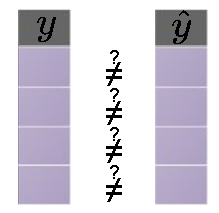
\includegraphics[width=0.9\textwidth]{figure_man/eval-classif-loss-compare-mce.pdf}
\textbf{ACC}
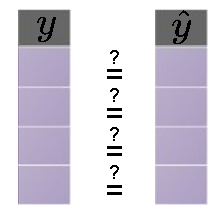
\includegraphics[width=0.9\textwidth]{figure_man/eval-classif-loss-compare.pdf}


\end{center}

\end{column}
\end{columns}



\end{vbframe}





\begin{vbframe}{Labels: Confusion Matrix}
% 
% True classes in columns.\\
% Predicted classes in rows.\\

\lz

\begin{table}[]
\centering
\begin{tabular}{cc|cccc|c|}
& \multicolumn{6}{c}{True classes} \\ 
\hline
& &\textbf{setosa} & \textbf{versicolor} & \textbf{virginica} & \textbf{error} & \textbf{$n$} \\ 
\hline

\multirow{4}{*}{\rotatebox[origin=c]{90}{\parbox{1.5cm}{Predicted \\ classes}}}   

& \textbf{setosa}     & 50              & 0                   & 0                  & 0              & 50           \\
& \textbf{versicolor} & 0               & 46                  & 4                  & 4              & 50           \\
& \textbf{virginica}  & 0               & 4                   & 46                 & 4              & 50           \\
& \textbf{error}      & 0               & 4                   & 4                  & 8              &      -        \\
\hline
& \textbf{$n$}        & 50              & 50                  & 50                 &      -          & 150          \\ 

%& & & & & &\\

\hline
\end{tabular}
\end{table}
\lz
We can see class sizes (predicted and true) and where errors occur.
\end{vbframe}



\begin{vbframe}{Labels: Confusion Matrix}
\textbf{In binary classification}
% % FIGURE SOURCE: No source
% \includegraphics[width=0.7\textwidth]{figure_man/roc-confmatrix1.png}

\begin{center}
\small
\begin{tabular}{cc|>{\centering\arraybackslash}p{7em}>{\centering\arraybackslash}p{8em}}
    & & \multicolumn{2}{c}{\bfseries True Class $y$} \\
    & & $+$ & $-$ \\
    \hline
    \bfseries Pred.     & $+$ & True Positive (TP)  & False Positive (FP) \\
              $\yh$ & $-$ & False Negative (FN) & True Negative (TN) \\
\end{tabular}
\end{center}

\end{vbframe}




\begin{vbframe}{Labels: Costs}
We can also assign different costs to different errors via a cost matrix.

$$
  Costs = \meanin C[\yi, \yih]
$$

\underline{Example}: \\

Depending on certain features (age, income, profession, ...) a bank wants to decide, if it grants a 10,000 EUR loan.\\ 

\medskip

Predict if a person is solvent (yes / no).\\ 
Should a bank give her/him a loan?\\


\medskip
  \begin{tabular}{ll}
    \textbf{Examplary costs:} & \\
    Loan cannot be repaid:& 10,000 EUR\\
    Interest paid for the loan:& 100 EUR\\
 
  \end{tabular}
  


 \begin{table}[ht]
 \small

\begin{tabular}{cccc}
    \hline
    & &\multicolumn{2}{c}{True classes} \\ 
    & &\textbf{solvent} & \textbf{not solvent}  \\ 
 \hline
    \multirow{2}{*}{\parbox{1cm}{Predicted \\ classes}}& \textbf{solvent}     & 0                 & 10,000\\
    & \textbf{not solvent} & 100               & 0\\
    \hline
\end{tabular}

\end{table}
 


\end{vbframe}
%--------------------------------------------------------

\begin{vbframe}{Labels: Costs}

\begin{columns}
\begin{column}{0.5\textwidth} 
\footnotesize\textbf{Cost matrix}
 \begin{table}[ht]
 \tiny
\begin{center}
\begin{tabular}{cccc}
    \hline
    & &\multicolumn{2}{c}{True classes} \\ 
    & &\textbf{solvent} & \textbf{not solvent}  \\ 
 \hline
    \multirow{2}{*}{\parbox{0.5cm}{Predicted \\ classes}}& \textbf{solvent}     & 0                 & 10,000\\
    & \textbf{not solvent} & 100               & 0\\
    \hline
\end{tabular}
\end{center}
\end{table}
\end{column}

\begin{column}{0.5\textwidth}
\footnotesize\textbf{Confusion matrix}
 \begin{table}[ht]
 \tiny
\begin{center}
\begin{tabular}{cccc}
    \hline
    & &\multicolumn{2}{c}{True classes} \\ 
    & &\textbf{solvent} & \textbf{not solvent}  \\ 
 \hline
    \multirow{2}{*}{\parbox{0.5cm}{Predicted \\ classes}}& \textbf{solvent}     & 70                 & 3\\
    & \textbf{not solvent} & 7              & 20\\
    \hline
\end{tabular}
\end{center}
\end{table}
\end{column}
\end{columns}



 
  \begin{itemize}
    \item If the bank gives every person a credit, the costs are at:
      \begin{align*}
      Costs &= \meanin C[\yi, \yih] \\&= 
      \frac{1}{100} \left( 
      -37 \cdot 7 + 
      0 \cdot 0 + 
      3 \cdot 93 +
      0 \cdot 0 
      \right) = 0.2
    \end{align*}
    
  
  \end{itemize}
 
 
\end{vbframe}


\begin{vbframe}{Probabilities: Brier Score}
Measures squared distances of probabilities from the true class labels:
\[
BS1 = \meanin \left( \pixih - \yi \right)^2
\]


\begin{itemize}
  \item Fancy name for MSE on probabilities
  \item Usual definition for binary case, $\yi$ must be coded as 0 and 1.
\end{itemize}

\begin{knitrout}\scriptsize
\definecolor{shadecolor}{rgb}{0.969, 0.969, 0.969}\color{fgcolor}

{\centering \includegraphics[width=0.95\textwidth]{figure/eval_mclass_1} 

}



\end{knitrout}


\framebreak

\[
BS2 = \meanin \sumkg \left( \pikxih - o_k^{(i)} \right)^2
\]
\begin{itemize}
  \item Original by Brier, works also for multiple classes
  \item $ o_k^{(i)} = [ \yi = k ] $ is a 0-1-one-hot coding for labels
  \item For the binary case, BS2 is twice as large as BS1, because in BS2 we sum the squared
    difference for each observation regarding class 0 \textbf{and} class 1, not only the true class.
\end{itemize}


\end{vbframe}

\begin{vbframe}{Probabilities: Log-Loss}
Logistic regression loss function, a.k.a. Bernoulli or binomial loss, $\yi$ coded as 0 and 1.
\[
LL = \meanin \left( - \yi \log(\pixih) - (1-\yi) \log(1-\pixih) \right)
\]
\begin{knitrout}\scriptsize
\definecolor{shadecolor}{rgb}{0.969, 0.969, 0.969}\color{fgcolor}

{\centering \includegraphics[width=0.8\textwidth]{figure/eval_mclass_2}  

}



\end{knitrout}
\begin{itemize}
  \item Optimal value is 0, \enquote{confidently wrong} is penalized heavily
  \item Multiclass version: $ LL = - \meanin \sumkg o_k^{(i)} \log(\pikxih) $
\end{itemize}
\end{vbframe}


\endlecture
\end{document}
